
\documentclass[11pt,a4paper,slovene]{myarticle}

%Uporabljeni paketi
\usepackage[slovene]{babel}
\usepackage[utf8]{inputenc}
\usepackage{lmodern}
\usepackage[T1]{fontenc}
\usepackage{fancyhdr}
\usepackage{caption}
\captionsetup{font={default,footnotesize}, labelfont=bf, format=hang,indention=.0cm}
\usepackage{graphicx,epsfig}
\usepackage{amsmath}
\usepackage{multirow}
\usepackage{color}
\usepackage{url}
\usepackage{makeidx}
\usepackage{listings}
\usepackage[official]{eurosym}

\definecolor{dkgreen}{rgb}{0,0.6,0}
\definecolor{gray}{rgb}{0.5,0.5,0.5}
\definecolor{mauve}{rgb}{0.58,0,0.82}

\lstset{frame=tb,
  language=C++,
  aboveskip=3mm,
  belowskip=3mm,
  showstringspaces=false,
  columns=flexible,
  basicstyle={\small\ttfamily},
  numbers=none,
  numberstyle=\tiny\color{gray},
  keywordstyle=\color{blue},
  commentstyle=\color{dkgreen},
  stringstyle=\color{mauve},
  breaklines=true,
  breakatwhitespace=true,
  tabsize=3
}

\usepackage{hyperref}
\hypersetup{
   bookmarksnumbered=true,
   urlbordercolor={0 1 0},
   linkbordercolor={1 1 1},
   unicode=true,
   pdftitle={ Modeliranje Računalniških Omrežij },
   pdfauthor={Asistent},
   pdfdisplaydoctitle=true,
   pdftoolbar=true,
   pdfmenubar=true,
   pdfstartview=X Y Z
}

\urlstyle{same}

\setlength{\parskip}{12pt}
\setlength\parindent{0pt}
\setlength\unitlength{1mm}

\begin{document}
\label{naslov}
\pdfbookmark[1]{Naslov}{naslov}
\thispagestyle{empty}

\begin{center}
\begin{Large}
Modeliranje računalniških omrežij\\
Študijsko leto 2019/2020\\
\end{Large}

\vspace*{4cm}
\begin{LARGE}
\textbf{Naloga 4 - Modeliranje IPv6 omrežij\\}
\end{LARGE}
\vspace*{0.5cm}

\begin{Large}
Poročilo za drugo seminarsko nalogo\\

\vspace*{4cm}

Mihael Šinkec\\
Vpisna št. 63170277\\
Matej Fortuna\\
Vpisna št. 63170091\\
Matej Fajdiga\\
Vpisna št. 63170084\\
Dominik Skapin\\
Vpisna št. 63150262\\

\vspace*{2cm}
Ljubljana, \today
\end{Large}
\end{center}

\pagebreak
\setcounter{page}{1}
\pagenumbering{arabic}


\label{Kazalo}
\pdfbookmark[1]{Kazalo}{Kazalo}
\tableofcontents
\thispagestyle{empty}
\pagebreak

\section{Opis primerov IPv6 omrežij}
\subsection{Omrežje 1 - IPv6 N Clients}
To omrežje je sestavljeno iz n odjemalcev, strežnika in treh IPv6 usmerjevalnikov. Strežnik nudi dostop s telnet protokolom, preko katerega odjemalci dostopajo nanj.

\begin{figure}[h]
  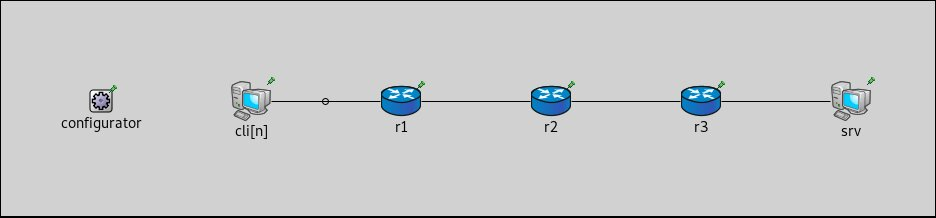
\includegraphics[width=\linewidth]{ipv6nclients.jpg}
\end{figure}

Število odjemalcev je nastavljivo preko parametra simulacije. Posameznemu odjemalcu je možno nastaviti določeno število aplikacij, ki tečejo na njem. V tem primeru na vsakemu odjemalcu teče po en telnet program/odjemalec.
telnet programu je moč tudi dodeliti poseben port. Ta je privzeto nastavljen na vrednost 1000. Nastavi se tudi IPv6 naslov strežnika, ter port telnet programa, ki teče na njem. Nato se programu nastavijo ostali parametri, kot so število poslanih ukazov, hitrost tipkanja, itd.. Primer konfiguracije izgleda takole:

\begin{lstlisting}
# tcp apps
**.cli[*].numApps = 1
**.cli[*].app[*].typename = "TelnetApp"
**.cli[*].app[0].localAddress = ""
**.cli[*].app[0].localPort = 1000
#IP address intentionally set incorrectly
**.cli[*].app[0].connectAddress = "srv[1]"
#**.cli[*].app[0].connectAddress="aaaa:2a:1:0:8aa:ff:fe00:dddd"
**.cli[*].app[0].connectPort = 1000

**.cli[*].app[0].startTime = uniform(10s,15s)
**.cli[*].app[0].numCommands = int(exponential(10))
**.cli[*].app[0].commandLength = intWithUnit(exponential(10B))
**.cli[*].app[0].keyPressDelay = exponential(0.1s)
**.cli[*].app[0].commandOutputLength = intWithUnit(exponential(40B))
**.cli[*].app[0].thinkTime = truncnormal(2s,3s)
**.cli[*].app[0].idleInterval = truncnormal(3600s,1200s)
**.cli[*].app[0].reconnectInterval = 30s
\end{lstlisting}

TODO: Opiši vrednosti

Podobno je možno konfigurirati aplikacije, ki tečejo na strežniku:
\begin{lstlisting}
**.srv[*].numApps = 1
**.srv[*].app[*].typename = "TcpGenericServerApp"
**.srv[*].app[0].localAddress = ""
**.srv[*].app[0].localPort = 1000
**.srv[*].app[0].replyDelay = 0s
\end{lstlisting}

TODO: Opiši vrednosti

Nastaviti je potrebno tudi omrežne vmesnike (NIC) na napravah:
\begin{lstlisting}
# Ethernet NIC configuration
**.eth[*].queue.typename = "EtherQosQueue"
**.eth[*].queue.dataQueue.typename = "DropTailQueue" # in routers
**.eth[*].queue.dataQueue.frameCapacity = 10  # in routers
**.eth[*].mac.duplexMode = true
\end{lstlisting}

TODO: Opiši vrednosti

Povezave (na 2. nivoju po TCP/IP) med posameznimi napravami se lahko nastavijo na Ethernet oz. na PPP protokol.
V tej implementaciji to ni možno narediti preko .ini parametrov, saj je treba v NED datoteki omrežja uvozit posebni tip povezave. Zato je potrebno ustvariti posebej NED datoteko za ethernet, kot tudi za PPP.
Tej povezavi lahko definiramo hitrost prenosa ter latenco.

Primer za ethernet:
\begin{lstlisting}
channel ethernetline extends DatarateChannel
{
    delay = 0.1us;
    datarate = 100Mbps;
}
\end{lstlisting}

Posamezne naprave nato povežemo z definirano povezavo:
\begin{lstlisting}
 connections:
        for i=0..n-1 {
            cli[i].ethg++ <--> ethernetline <--> r1.ethg++;
        }
        r1.ethg++ <--> ethernetline <--> r2.ethg++;
        r2.ethg++ <--> ethernetline <--> r3.ethg++;
        r3.ethg++ <--> ethernetline <--> srv.ethg++;
\begin{lstlisting}

Ko simuliramo omrežje se simulira vse od povezavni plasti gor do aplikacijske plasti, tj. od ethernet/PPP okvirjev, do telnet paketov. Pri vizualizaciji seveda vidimo samo okvirje, ker so paketi tudi del teh okvirjev.




\subsection{Omrežje 2 - IPv6 Bulk Transfer}
Tukaj piši, Matej, in zavrti kolo.......


\end{document}











